
\documentclass[11pt,a4paper]{CLabBookTemplate} %load the style file for the Extended Essay

\addbibresource{MyBibliography.bib} %specifying the bibliography file

% information about you and the document
\author{Tim Meiwald}
 %000017-0104 -> candidate number
\usepackage{multicol}


% For the C code snippets
\usepackage{listings}
\usepackage{xcolor}


\definecolor{mGreen}{rgb}{0,0.6,0}
\definecolor{mGray}{rgb}{0.5,0.5,0.5}
\definecolor{mPurple}{rgb}{0.58,0,0.82}
\definecolor{backgroundColour}{rgb}{0.95,0.95,0.92}

\lstdefinestyle{CStyle}{
	backgroundcolor=\color{backgroundColour},   
	commentstyle=\color{mGreen},
	keywordstyle=\color{magenta},
	numberstyle=\tiny\color{mGray},
	stringstyle=\color{mPurple},
	basicstyle=\footnotesize,
	breakatwhitespace=false,         
	breaklines=true,                 
	captionpos=b,                    
	keepspaces=true,                 
	numbers=left,                    
	numbersep=5pt,                  
	showspaces=false,                
	showstringspaces=false,
	showtabs=false,                  
	tabsize=2,
	language=C
}

\lstset{language=C}




\title{MA4080 - Computational Task 1 } % use capitals


% \component{Electronic Lab Book} % or Lab report, Exploration, etc
% \session{Year 1 Semester 1}

% \wordcount{xxxx} %change this to the actual number

\usepackage{graphicx}

\begin{document}

\pagenumbering{roman} %roman page numbers to be used on the title, abstract, acknowledgment and contents page
\setcounter{page}{1} % start with page 1

\maketitle % generating the title page




% Generating the table of contents
\thispagestyle{fancy} % put the required information in the header
\addcontentsline{toc}{section}{Contents} % include this in the table of contents
\mytableofcontents
\newpage % Start the main text on a new page


% Here comes the important part, the main text
\pagenumbering{arabic} % arabic page numbers to be used from now on
\setcounter{page}{1} % start again with page 1

\section{Logistic Map - Discrete Time Logistic Equation}

The discrete time logistic equation  as given in Equation \ref{LogisticMap} represents the discrete-time equivalent of the logistic equation first developed by Pierre-Fran\c cois Verhulst. \par 

\begin{equation}
\label{LogisticMap}
P_{N+1} = rP_{N}\left(1 - \frac{P_{N}}{K}\right)
\end{equation}

It describes how the population changes per time step given that there is some growth rate, r and some carrying capacity, K. The growth rate, r describes how fast the population grows when there are sufficient resources available for the population to grow. While the carrying capacity, K describes the maximum population that can exist given the available resources. \par
The equation is sensitive in it's behaviour to the value of r. The equation either gives a decaying population, an increasing population until remaining stable at some point, oscillating between various points in a stable cycle, chaotic behaviour or at r$>$4 a relatively meaningless result where one can end up with negative population levels which would clearly be unphysical. \par
As such it models demographic growth or other phenomena such as the GDP growth of a nation albeit often not particularly well. However, how growth differs from the equation can give us an approximate idea of where to look in terms of what to add to the model to improve it. For example, we could use the equation to model the GDP growth of a nation for periodic intervals of years. If the real results are less than the model we could expect to look for some external factors that inhibited growth while if it is more than the model we could expect to look for something that increased growth in that time period. \par
Part of the issues that arise with using this equation is it's sensitivity to the value of r. In particular, in real world processes it is not always possible to establish an exact value of r. Which means that the uncertainty of r could in, for example the chaotic region, lead to wildly different results. While in the oscillating region it could lead to differences in the number of points the equation oscillates between or in the value thereof. This would in some situations be fairly consequential, for example mispredicting GDP growth in a nation can have major real world consequences when the prophecy fulfils itself by virtue of the market responding to the prediction itself. If given out by a suitably authoritative source such as a central bank. \par 

\begin{figure}
	\centering
	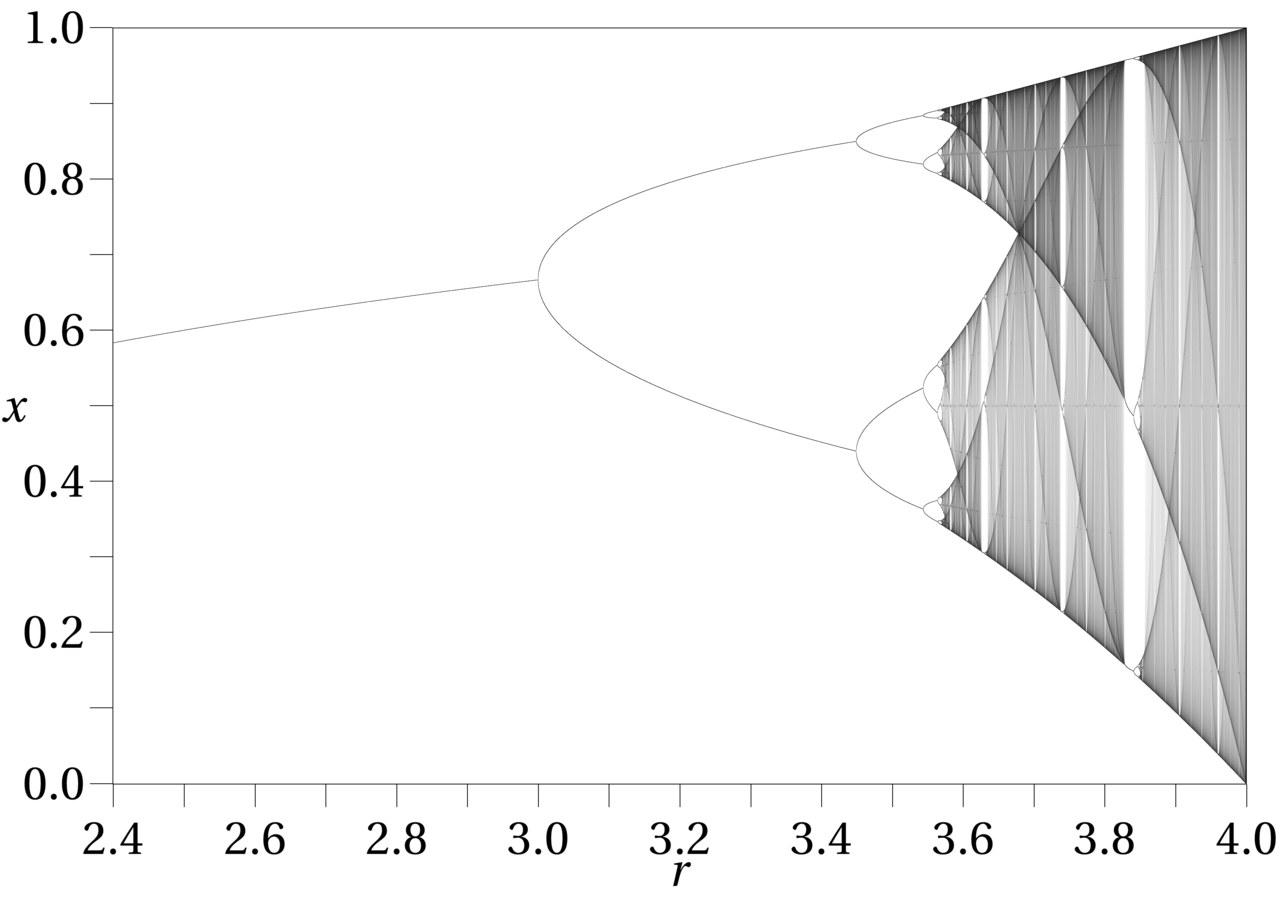
\includegraphics[width = 120mm]{Figures/LogisticBifurcationMap.png}[h!]
	\caption{Logistic Bifurcation Map \cite{LBM}. The Bifurcation map describes the change in behaviour of the Logistic map. Here we can see the range in which the Logistic map results in a stable equilibrium on the left side of the diagram, while in the middle part of the graph we can see that the Logistic map ends up in a stable cycle between various points while on the right side we can see that the Logistic map ends up being chaotic apart from the stable "island" at around r = 3.8}
	\label{fig:LogisticBifurcationMap}
\end{figure}

The bifurcation of the logistic map describes whether the logistic map results in a stable equilibrium. As we can see in Figure \ref{fig:LogisticBifurcationMap} the logistic map for smaller r values reaches a stable equilibrium around one point, while for larger r values it oscillates around 2,4 or more values while at very large r the logistic map ends up in a chaotic system. 

\newpage
\section{Logistic Map}
For K = 1 and and the initial starting value, P0 $\in$ [0.5,0.2,0.8] for the growth rate, r $\in$ [0.6, 1.7, 2.8, 3.2, 3.6, 3.9]. \par 

We can observe systematic behaviour when we change P0 as described in the section above. For growth rates, r $\in$ [0,1] the population collapses regardless of the initial value, P0. For growth rates, r $\in$ [0.6,1.7] the population stabilises around an equilibrium at approximately $\frac{r -1 }{r}$ while for growth rates, r = 3.2 the population oscillates between two values. For r = 3.6 and 3.9 the population levels become chaotic. We can see an example of this for P0 = 0.5 in Figure \ref{fig:LogisticMapP05}. The graphs for P0 = 0.2,0.8 behave similarly. With the only difference that in the initial transient state they obviously start at a different initial population. 
\begin{figure}[h!]
	\centering
	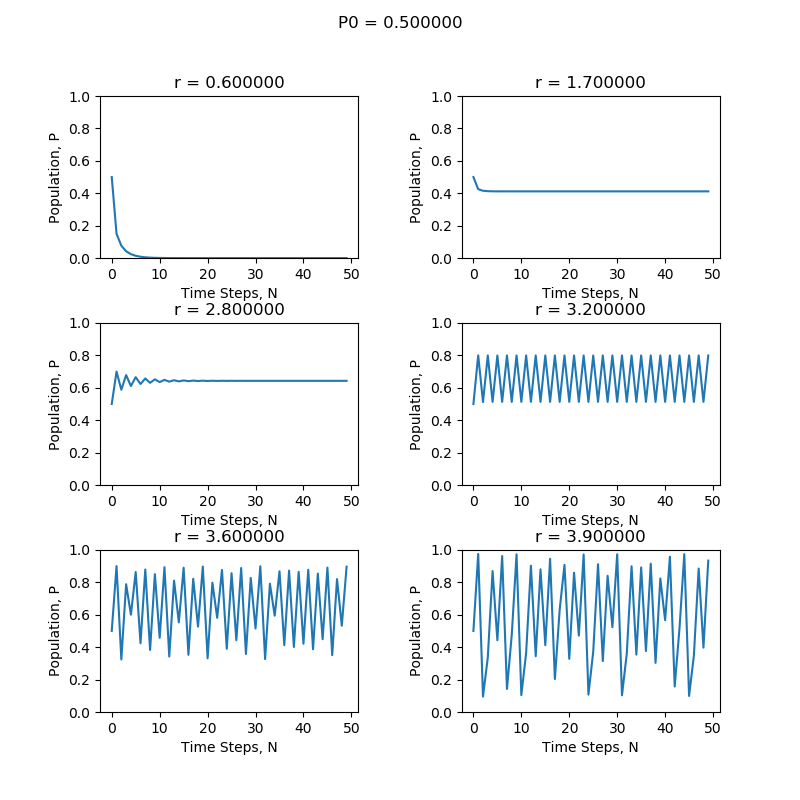
\includegraphics[width = 160mm]{Figures/DLMP0.png}
	\caption{The logistic map for the initial starting condition, P0 = 0.5 and the growth rate, $\in$  [0.6, 1.7, 2.8, 3.2, 3.6, 3.9] }
	\label{fig:LogisticMapP05}
\end{figure}

As we can see in Figure \ref{fig:LogisticMapr3.2}, the equilibrium state for the logistic map remains the same regardless of initial population level. And is only dependent on r. While of course, the transient state is affected by the difference in initial population level. 
\begin{figure}[h!]
	\centering
	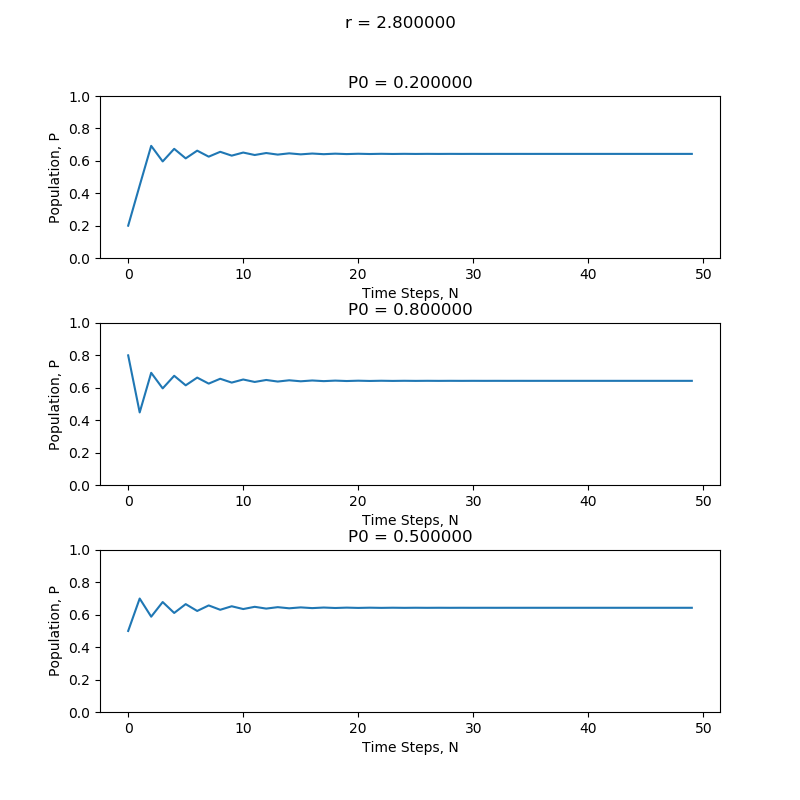
\includegraphics[width = 120mm]{Figures/DLMr3.png}
	\caption{The logistic map for the growth rate, r = 2.8 for varying initial population levels, P0. As we can see quite clearly, regardless of initial population level all the populations reach the same equilibrium level for the same r value. However, they do not behave the same for r in the chaotic regions.}
	\label{fig:LogisticMapr3.2}
\end{figure}
In the chaotic region, as seen in Figure \ref{fig:LogisticMapr3.9} the initial population level, P0 affects the behaviour throughout the graph due to it being chaotic and as such the behaviour can vary drastically based on the initial conditions. 
\begin{figure}[h!]
	\centering
	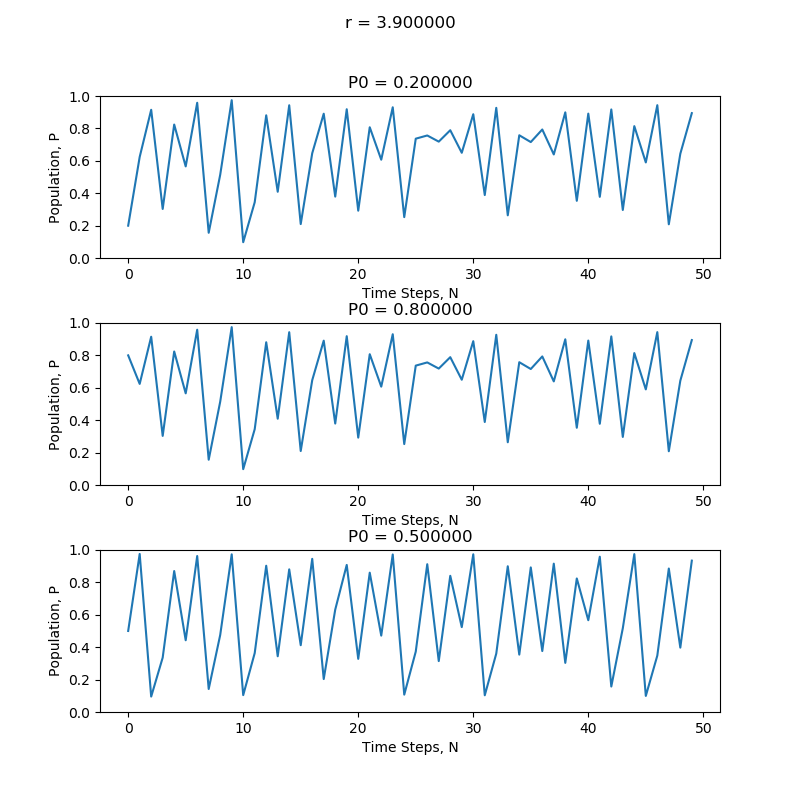
\includegraphics[width = 120mm]{Figures/DLMr6.png}
	\caption{The logistic map for the growth rate, r = 3.9 for varying initial population levels, P0. As we can see quite clearly,The behaviour is chaotic and it's behaviour varies depending on the initial population level, P0. Unlike for the r values less than 3 where they all stabilise or oscillate around the same value, or in the case of r $<$ 1, the populations all collapse.}
	\label{fig:LogisticMapr3.9}
\end{figure}

From Figures \ref{fig:LogisticMapP05},\ref{fig:LogisticMapr3.2} and \ref{fig:LogisticMapr3.9} we can tell that the discrete map can, depending on the growth rate be relatively similar to the continuous logistic function for the situations in r leads to a smooth discrete map such as for r = 0.6 and 1.7, while being dissimilar for larger r, where the logistic map is no longer smooth but still somewhat like a continous logistic function in that it can oscillate between values. While for very large r such as r = 3.6 and 3.9 the discrete logistic map no longer acts like a continuous logistic function due to it's chaotic behaviour. \par 
Not all graphs generated have been included for the sake of brevity. 

\clearpage
\newpage
\section{Investigating World GDP}
As we can see in Figure \ref{fig:WorldGDP}, From the 1960s to the 1980s the World economy generally grew and then stagnated from 1980 to 1984. It then continued growing from 1985 to 1996 where it stagnated again until 2003. It then continued growing until 2007 where there was a financial crisis from 2007-2008. It then continued growing until 2014 where there was once again a financial crisis until 2015 at which point it continued growing again. Unfortunately, due to the nature of the graph, it is harder to see whether there are financial crises in the earlier years because of their relatively small changes compared to later years. For example, we know the Nixon shock happened in 1971 ushering in the stagflation in the early 1970s but this is difficult to see in the trend on the graph. Ideally, one would analyse each decade individually to see the smaller microtrends that existed. 

\begin{figure}[h!]
	\centering
	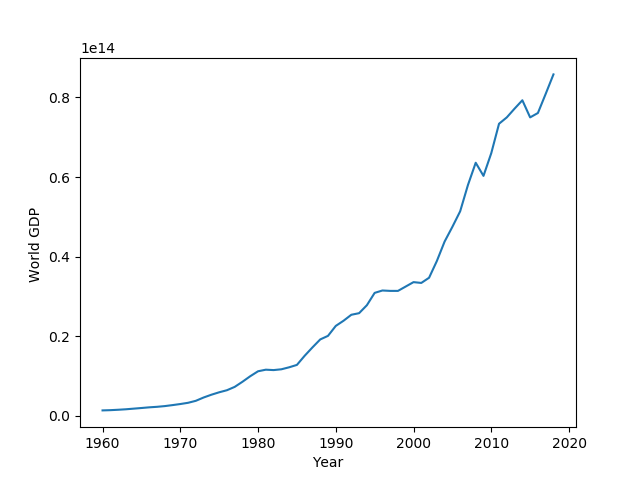
\includegraphics[width = 120mm]{Figures/WorldGDP.png}
	\caption{World GDP by year.}
	\label{fig:WorldGDP}
\end{figure}

The scatter plot of each value of the world GDP $P_{N}$ against $\frac{P_{N+1}}{P_{N}}$ is in Figure \ref{fig:WorldGDPScatter}. In this we can quite clearly see that the Logistic map does a terrible job of describing global economics. Since qualitatively, we can see that the points are not close to the regression line in general and quantitatively the fraction of variance unexplained, given as FVU in the graph is 0.82. Since the fraction of variance unexplained when equal to 1 implies that all of the variance is unexplained and at 0 implies that the variance is fully explained by the logistic map then our value implies that most, though not all, of the variance is not explained by this model. 

\begin{figure}[h!]
	\centering
	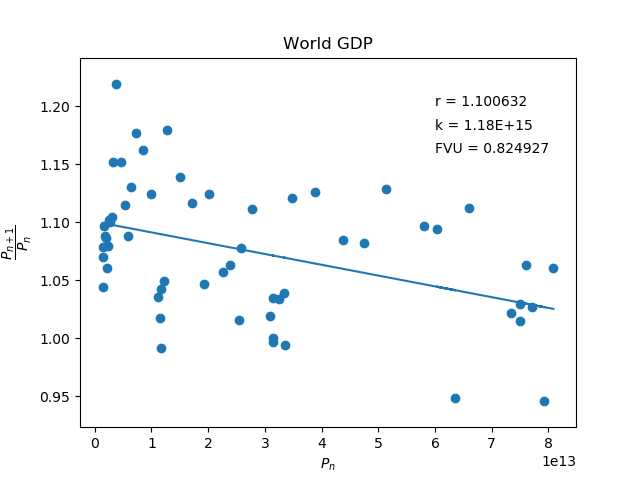
\includegraphics[width = 120mm]{Figures/WorldGDPScatter.png}
	\caption{The GDP value of the world plotted against the next years GDP value divided by the original years GDP value. With a linear regression line drawn in order to illustrate how well the Logistic map can describe global economics. The r and k value calculated from the linear regression values and the Fraction of Variance Unexplained, FVU are also given.}
	\label{fig:WorldGDPScatter}
\end{figure}


\begin{table}[h!]
	\begin{tabular}{|l|l|l|l|l|l|l|l|}
		\hline
		Year & 1960-1970 & 1971-1980 & 1981-1990 & 1991-2000 & 2001-2010 & 2011-2018 & 1960-2018   \\ \hline
		r    & 1.03726   & 1.16945   & 0.981953  & 1.23915   & 1.1982    & 1.50717   & 1.100632017 \\ \hline
		k    & -4.65E+13 & 3.32E+14  & -1.50E+14 & 1.77E+14  & 4.63E+14  & 2.40E+14  & 1.1814E+15  \\ \hline
		FVU  & 0.777408  & 0.975452  & 0.912757  & 0.703079  & 0.783525  & 0.65156   & 0.824926944 \\ \hline
	\end{tabular}
	\caption{Table providing the World GDP r,k and fraction of variance unexplained,FVU values for the time periods. Unfortunately, some k values are negative because the unexplained variance in the data dominates over the general trend leading to a negative k value. This is unphysical, since the carrying capacity cannot, by definition be less than zero. Since that would imply that the maximum sustainable economic production is negative. Which isn't possible. }
	\label{Task1Table}
\end{table}

\begin{figure}[h!]
	\centering
	\includegraphics[width = 120mm]{Figures/RgkWorld.png}
	\caption{The growth rate,r, the carrying capacity, k and the fraction of variance unexplained, FVU. For each decade. The horizontal lines are the value of r,g and FVU for the entire time period. Uses the data from Table \ref{Task1Table}}
	\label{fig:RgkWORLD}
\end{figure}

As we can see in Figure \ref{fig:RgkWORLD}. The growth rate r for each time interval of a decade can vary from the average over the whole time interval depending on whether GDP was growing, stagnating or reducing. The carrying capacity, k is much larger for the entire time interval than for each individual time interval. This is likely because the carrying capacity assumes there is some hard limit which prevents the world economy growing more than a certain amount. So this value is smaller for small time intervals because it implies that the end of the small time interval will approach the carrying capacity. While for the larger interval k must be much larger because it starts at a much smaller GDP, P0 and ends at a far higher GDP than for each individual time interval. \par
However, k increases from the 1970s to the 1980s implying the global economic capacity to do work increases but in the 1980s it decreases again, due to the recession which implies that it caused long term damage to economic capacity rather than a mere slowdown of the economy. \par
The Fraction of variance unexplained values, FVU, vary around the value for the entire time period. Simply because for some time periods the general trend is more obvious and as such the linear regression fits better, while for some the trend in that decade isn't obviously noticeable and as such has a far worse FVU than over the entire time interval. 

\clearpage
\section{Investigating Norwegian and South African GDP}
\subsection{Norway}

\begin{figure}[h!]
	\centering
	\includegraphics[width = 120mm]{Figures/NorGDP.png}
	\caption{GDP of Norway from 1960-2018}
	\label{fig:NorGDP}
\end{figure}

As we can see from Figure \ref{fig:NorGDP}, Norwegian GDP grew until the 1980's where it stagnated until 1985. It then grew turbulently until 1992 whereupon there was a recession until 1993. It then grew again until 1997 where there was another recession. It then grew until 2008 whereupon it crashed in 2009 then grew again in 2010 until 2014 where it again collapsed. The volatility in Norwegian GDP is likely not due to GDP changes in and of itself but because the GDP is in units of current US\$. For example, in the recession seen in 1992-1993 oil prices had collapsed forcing a devaluation of the Krone due to Norway's large reliance on oil revenue. So it appeared that Norway's GDP shrank because it no longer provided as much "value" by selling oil, but largely because oil wasn't worth as much anymore and not because of lack of productivity. Hence, why Norway then bounces back rapidly as oil prices recovered. 


\begin{figure}[h!]
	\centering
	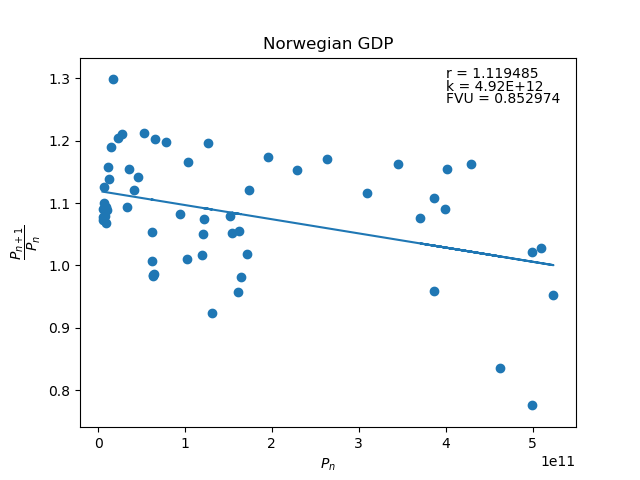
\includegraphics[width = 120mm]{Figures/NORGDPScatter.png}
	\caption{The GDP value of Norway plotted against the next years GDP value divided by the original years GDP value. With a linear regression line drawn in order to illustrate how well the Logistic map can describe global economics. The r and k value calculated from the linear regression values and the Fraction of Variance Unexplained, FVU are also given.}
	\label{fig:NORGDPScatter}
\end{figure}

Again due to the Fraction of variance unexplained, being nearer 1 than 0. The variance is largely unexplained by the model. This can be seen graphically as the data values are distributed around the regression line rather than mapping closely to it. 
In general, Norway had a larger growth rate than the World as a whole since the 1950s. Since r is larger by approximately 0.1. This is to be expected given that Norway was a, by western standards, poor country in the 1950's and is now one of the richest countries partially due to the oil found in the North sea in the late 1960's. The k value drops from the 1960s until the 1980s at which point it increases again, which implies that the carrying capacity of the Norwegian economy decreased in those decades, at which point it picked up again. 

\begin{table}[h!]
	\begin{tabular}{|l|l|l|l|l|l|l|l|}
		\hline
		Year & 1960-1970 & 1971-1980 & 1981-1990 & 1991-2000 & 2001-2010 & 2011-2018 & 1960-2018   \\ \hline
		r    & 1.09597   & 1.29605   & 1.03098   & 1.30601   & 1.32179   & 1.39764   & 1.119485337 \\ \hline
		k    & 1.09E+12  & 3.24E+11  & -2.22E+12 & 6.92E+11  & 1.87E+12  & 1.62E+12  & 4.92418E+12 \\ \hline
		FVU  & 0.989576  & 0.49301   & 0.993005  & 0.842584  & 0.596358  & 0.78964   & 0.85297378  \\ \hline
	\end{tabular}
	\caption{Table providing the Norwegian GDP r,k and fraction of variance unexplained, FVU values for the time periods. Unfortunately, some k values are negative because the unexplained variance in the data dominates over the general trend leading to a negative k value. This is unphysical, since the carrying capacity cannot, by definition be less than zero. Since that would imply that the maximum sustainable economic production is negative. Which isn't possible.}
	\label{NorTable}
\end{table}
\clearpage

\begin{figure}[h!]
	\centering
	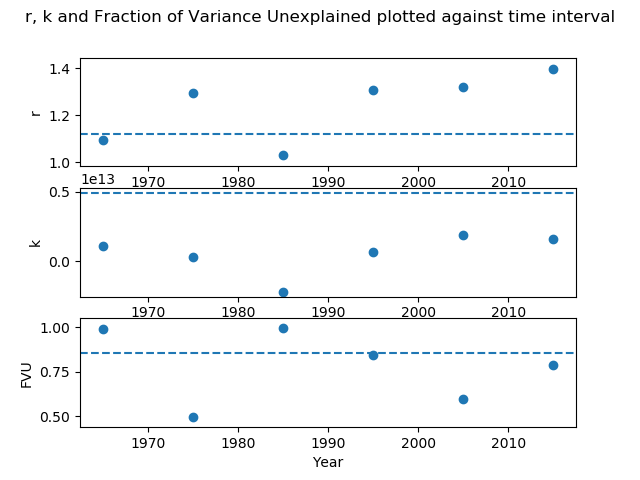
\includegraphics[width = 120mm]{Figures/RgkNOR.png}
	\caption{The growth rate,r, the carrying capacity, k and the fraction of variance unexplained, FVU. For each decade. The horizontal lines are the value of r,g and FVU for the entire time period. Uses the data from Table \ref{NorTable}}
	\label{fig:RgkNOR}
\end{figure}





\subsection{South Africa}
\begin{figure}[h!]
	\centering
	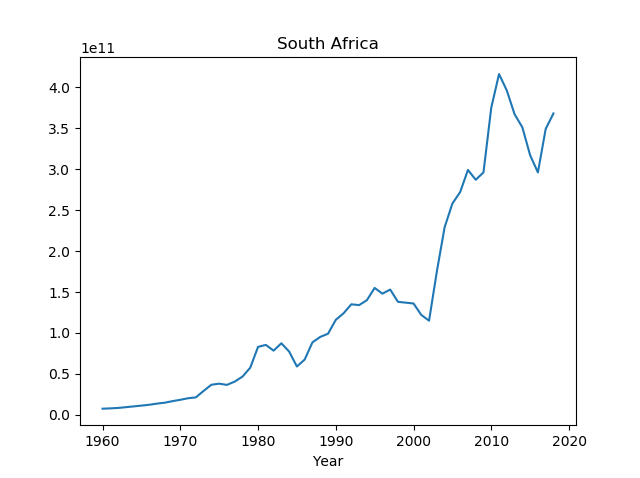
\includegraphics[width = 120mm]{Figures/RSAGDP.png}
	\caption{GDP of South Africa from 1960-2018}
	\label{fig:RSAGDP}
\end{figure}

As we can see in Figure \ref{fig:RSAGDP}. The GDP grows until 1972, where it accelerates somewhat until 1975, then plateaus until 1977 then increases again until 1980, where it stagnates until 1984 and then crashes in 1985. It then proceeds to grow again until 1996 and then becomes smaller until 2004 likely due to the period of global stagnation. It then grows until 2012 where it crashes again until 2015 due to the global recession and then starts growing again. 
\begin{figure}[h!]
	\centering
	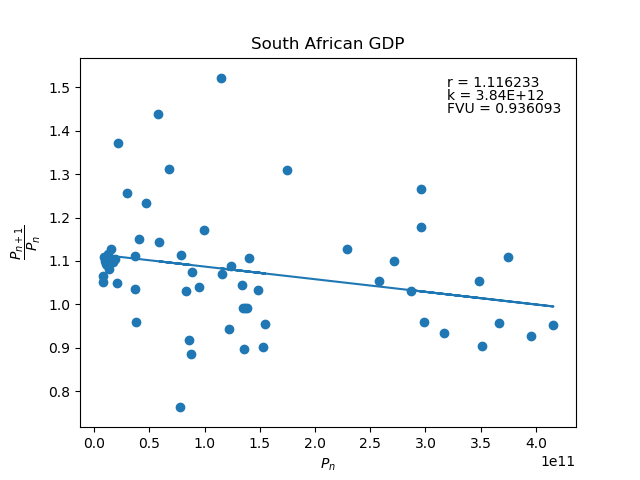
\includegraphics[width = 120mm]{Figures/RSAGDPScatter.png}
	\caption{The GDP value of South Africa plotted against the next years GDP value divided by the original years GDP value. With a linear regression line drawn in order to illustrate how well the Logistic map can describe global economics. The r and k value calculated from the linear regression values and the Fraction of Variance Unexplained, FVU are also given. Unfortunately, some k values are negative because the unexplained variance in the data dominates over the general trend leading to a negative k value. This is unphysical, since the carrying capacity cannot, by definition be less than zero. Since that would imply that the maximum sustainable economic production is negative. Which isn't possible.}
	\label{fig:RSAGDPScatter}
\end{figure}
Again the Fraction of variance unexplained is high and as such the model does not explain well any trends for the entire period. The growth rate is also very close to the global value. 

\begin{table}[]
	\begin{tabular}{|l|l|l|l|l|l|l|l|}
		\hline
		Year & 1960-1970 & 1971-1980 & 1981-1990 & 1991-2000 & 2001-2010 & 2011-2018 & 1960-2018   \\ \hline
		r    & 1.03426   & 1.26252   & 1.55107   & 1.63797   & 1.4538    & 1.40905   & 1.116232881 \\ \hline
		k    & -1.89E+11 & 3.66E+11  & 2.38E+11  & 3.70E+11  & 9.88E+11  & 1.24E+12  & 3.83532E+12 \\ \hline
		FVU  & 0.639375  & 0.94343   & 0.79616   & 0.535111  & 0.693471  & 0.801064  & 0.936093057 \\ \hline
	\end{tabular}
	\caption{Table providing the South African GDP r,k and fraction of variance unexplained, FVU values for the time periods}
	\label{RSATable}
\end{table}
For some of the decades in Table \ref{RSATable} and Figure \ref{fig:RgkRSA} the FVU is much better than the average for the overall period. Again this is due to the trend being more clear for smaller time periods. The r values are higher during periods of growth and lower for periods of stagnation. The k value increases over time. Which implies that the capacity of the economy to do work keeps increasing. Even if GDP itself shrinks. 
\begin{figure}[h!]
	\centering
	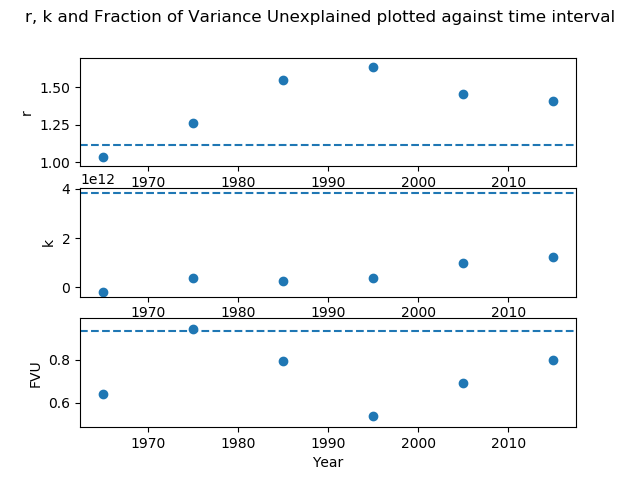
\includegraphics[width = 120mm]{Figures/RgkRSA.png}
	\caption{The growth rate,r, the carrying capacity, k and the fraction of variance unexplained, FVU. For each decade. The horizontal lines are the value of r,g and FVU for the entire time period. Uses the data from Table \ref{RSATable}}
	\label{fig:RgkRSA}
\end{figure}
\clearpage
\section{Simulation of Time series}
In this section we use the Discrete Logistic map to simulate the time series for the World, Norway and South Africa. We use the discrete logistic map over the whole period as the simulation. Quantitatively we could evaluate the accuracy by using the Fraction of variance unexplained between the model and the data points. Qualitatively, we evaluate the accuracy as terrible because the fundamental assumptions of this model are simply wrong. The assumption being that there exists a carrying capacity for the economy. This is, however, not the case. Since, the economic value of any product or service is entirely dependent on the value assigned to it by the consumer. And since, for example, services have no inherent resource limitation bar the energy needed to provide that service. And given that, current energy consumption is ~ 162 PWh \autocite{IEA} with a global maximum energy supply of 420 to 14000 PWh \autocite{UN}. We can see that the only fundamental limit is sufficiently far enough away for any current GDP growth to not be constrained by any carrying capacity. \newline
In addition, we were asked to simulate the economy using the smaller time intervals. Unfortunately, due to how badly the data maps to the model some values for the carrying capacity, k were evaluated to be negative. This is unphysical. Since the carrying capacity cannot by definition be less than 0. Even if we assumed a nuclear apocalypse that rendered Earth inhabitable the economic carrying capacity would be at minimum 0. So the smaller time series were not evaluated. 

\begin{figure}[h!]
	\centering
	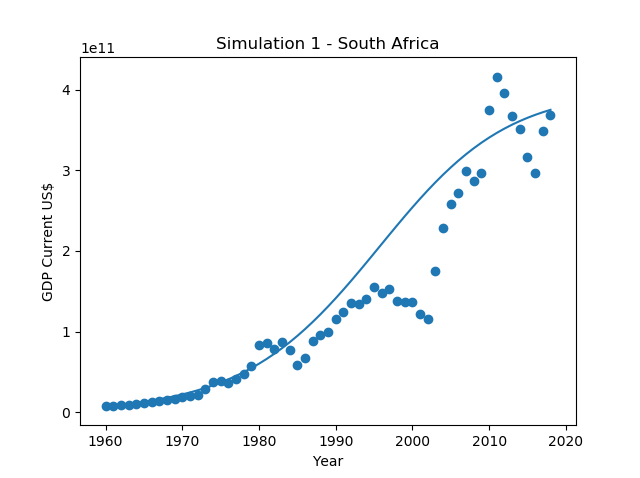
\includegraphics[width = 120mm]{Figures/RSASim.png}
	\caption{Scatter plot of GDP values of South Africa with the discrete logistic map of the growth rate, r and carrying capacity k of the entire time interval used to simulate the GDP for the whole time interval.}
	\label{fig:RSASim}
\end{figure}
\begin{figure}[h!]
	\centering
	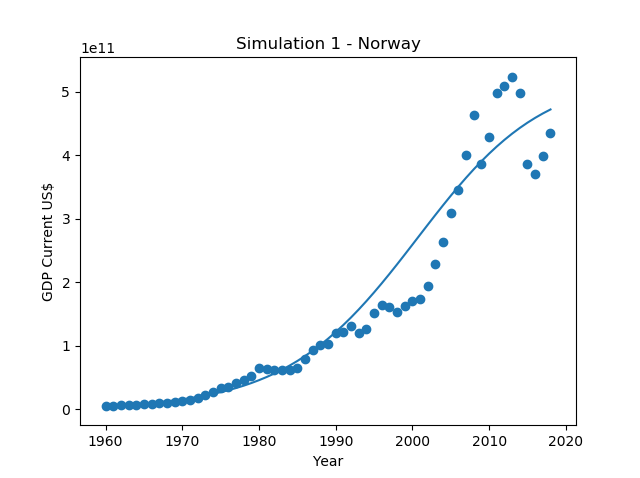
\includegraphics[width = 120mm]{Figures/NORSim.png}
	\caption{Scatter plot of GDP values of Norway with the discrete logistic map of the growth rate, r and carrying capacity k of the entire time interval used to simulate the GDP for the whole time interval.}
	\label{fig:NORSim}
\end{figure}
\begin{figure}[h!]
	\centering
	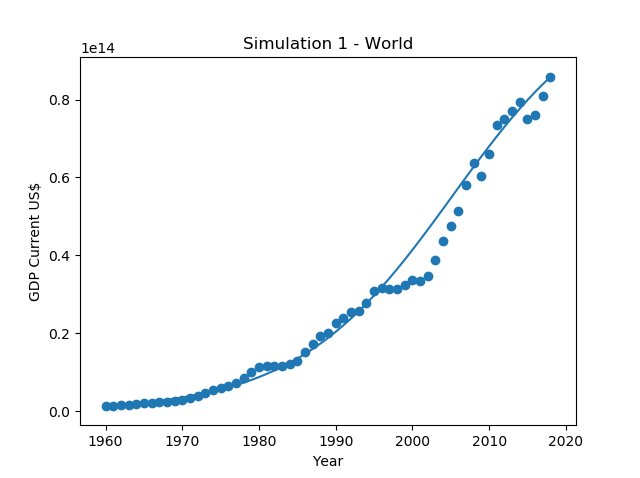
\includegraphics[width = 120mm]{Figures/WorldSim.png}
	\caption{Scatter plot of GDP values of the world with the discrete logistic map of the growth rate, r and carrying capacity k of the entire time interval used to simulate the GDP for the whole time interval.}
	\label{fig:WorldSim}
\end{figure}


\clearpage
\printmybibliography
\end{document}